\chapter{Design}
\label{chap:design}

\section{Choice of a consensus protocol}

One of the earliest solution to the consensus problem is Lamport's Paxos algorithm\cite{paxos}.
It is currently widely used, for example Google relies on it a lot to ensure correctness of its distributed systems\cite{chubby, paxoslive}.
However, Paxos has two issues: first, it only solves part of the problem; some other ``bricks'' must be added to it to form a complete system.
In addition to this, Paxos is known to be hard to understand, and even more to implement correctly.
Most of its users rely on pre-existing implementations such as libpaxos\footnote{\url{https://bitbucket.org/sciascid/libpaxos/}}.
This means modifying the consensus protocol for our application and chosent transport could be hard to do

Fortunately for us, a simpler alternative to Paxos called Raft was recently introduce\cite{raft}.
Raft was designed from the ground up to be simpler by cleanly separating the different parts of the problem.
It also provides a complete solution, unlike Paxos which often requires additional, unproven extension\cite{paxoslive}.

Another possible choice would have been ZooKeeper's ZAB\cite{zookeeper}, but was not as well documented as Raft.
In addition, it appeared to provide primitives that were less general purposes than a replicated log.

Despite the availability of excellent production grade Raft implementations, we decided to implement our own.
Most existing Raft implementations are using high level languages such as Go, which are not suited for low latency programming.
Other implementations in C or C++ make a lot of hypothesis on the underlying platform.
For all those reasons, it was deemed easier to do it ourself, using experience gathered by doing a prototype in Python.
The resulting implementation is pretty small, at about 1000 lines of C++ code.

\section{Modifications to R2P2}


\begin{figure}[h]
    \centering
    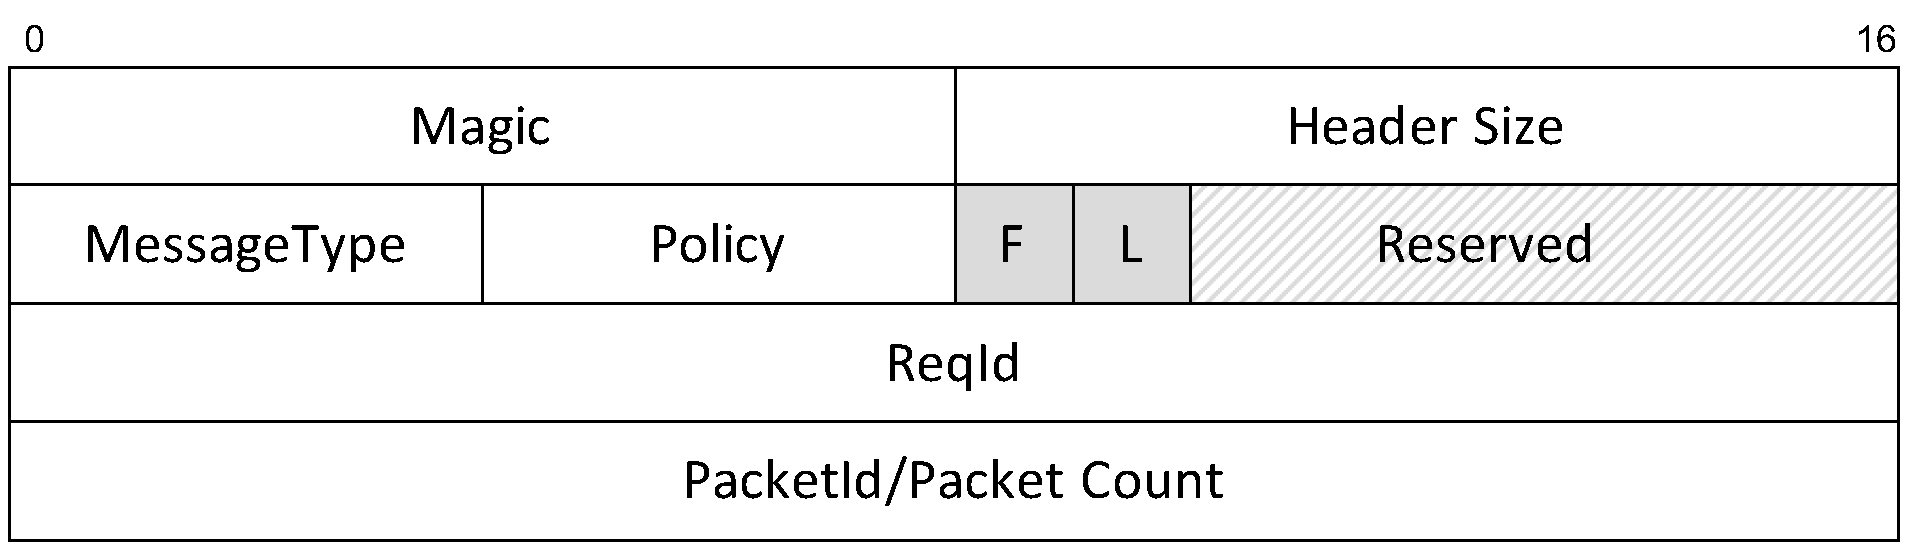
\includegraphics[width=0.6\textwidth]{r2p2_header}
    \caption{\gls{r2p2} header format\cite{r2p2}}
    \label{fig:r2p2-header}
\end{figure}


Fortunately for us, \gls{r2p2} requests have a \emph{Policy} field to indicate to load balancers how this request should handled (Figure~\ref{fig:r2p2-header}).
The pre-existing policies were \texttt{LB\_ROUTE} (can be redirected to any backend) or \texttt{FIXED\_ROUTE} (the request should really be handled by the destination backend).
We added the \texttt{REPLICATED\_ROUTE} policy: all the backends will eventually receive this request.
In addition, all backends are guaranteed to receive the requests using this policy in the same order.

Since this policy field is per request, it means clients can selectively enable request replication.
For example, a user might specify that no write should be lost but that stale reads are acceptable (to lower latency).
Then write requests would be sent with the \texttt{REPLICATED\_ROUTE} policy, while reads are sent with \texttt{LB\_ROUTE}.

Another addition to the R2P2 protocol was to add a new \emph{MessageType} for Raft-related messages.
The different types of Raft messages are differentiated in the payload of the message.

\section{Request lifecycle}

\begin{figure}[hp]
    \centering
    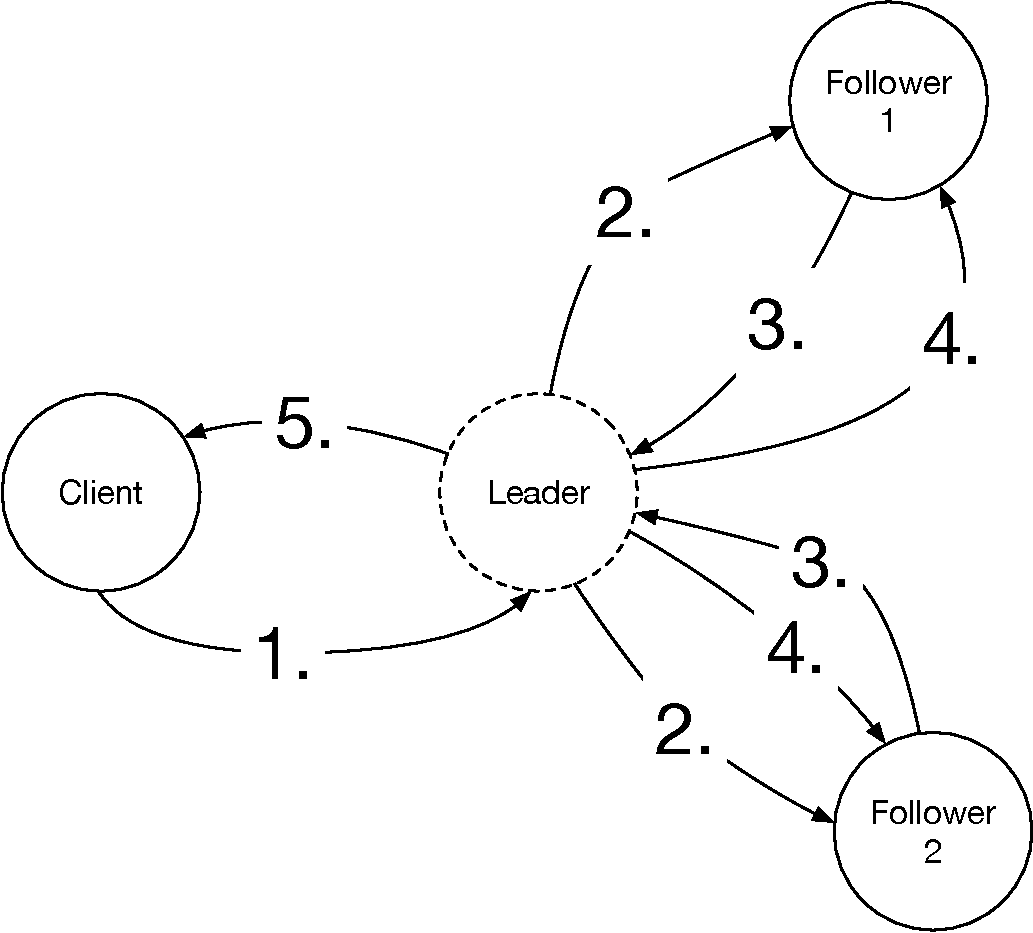
\includegraphics[width=0.8\textwidth]{client_server_interaction}
    \caption{Typical client server interaction for a replicated service call.
        Request arrives to the leader (1).
        Request is then replicated to all followers (2).
        Followers acknowledge the replication (3).
        Leader marks the request committed (4).
        Commited requests are forwarded to the application and replies are sent to the client (5).
    \label{fig:client-server-interaction}
    }
\end{figure}

Figure~\ref{fig:client-server-interaction} shows how a replicated request is handled.
In this example, the first node is the leader, and therefore the request must be directed to it (1).
The request is then packed in a log entry, and sent to the followers through Raft's \emph{AppendEntryRequest} message (2).
Nodes then send back an \emph{AppendEntryReply} message, acknowledging the message to the leader (3).
Once a request has been acknowledged by a majority of the nodes, the leader marks it as committed.
From this point on, the request will not be lost by the cluster\footnote{Provided that a majority of nodes stay healthy}.
Therefore, the request is forwarded to the application and the reply sent to the client (5).
On next message, or on timeout, the new commit index will also be sent to followers (4).
At this point they also forward it to their local copy of the application, which also sends back answers(5).

Having the followers send back a reply to the client ensures that the reply is sent in case of leader crash.
However, it will greatly increase the load on the network, which might be an issue.
One possible fix for this would be to have the followers run the request locally but drop the reply.

